\documentclass{article}
\usepackage{geometry}
\usepackage{graphicx}
\usepackage{amsmath}
\usepackage{hyperref}
\usepackage{listings}

\geometry{a4paper, margin=1in}

\title{Reinforcement Learning Project Report: Implementing and Analyzing RL Algorithms in MDP}
\author{[Noé Bourgeois]}
\date{\today}

\begin{document}

\maketitle

\section{Introduction}
This report presents the implementation and analysis of two key reinforcement learning algorithms: 
Value Iteration and Q-Learning within a Markov Decision Process (MDP) framework. 
This project extends foundational concepts from "2-adversarial" into a more complex, 
multi-agent setting, emphasizing algorithmic adaptability and robustness.

\section{Project Overview}
\subsection{Objective}
The objective of this project is to develop and analyze algorithms that can efficiently solve complex decision-making problems modeled as MDPs, 
with a focus on environments characterized by multiple agents and uncertain outcomes.

\subsection{Methodology}
The project methodology involves implementing the Value Iteration and Q-Learning algorithms, 
conducting experiments to evaluate their performance, and analyzing their behavior in various simulated environments.

\section{Implementation}
\subsection{Value Iteration}
The Value Iteration algorithm was implemented following the Bellman Equation. 
This iterative process updates the value of each state until it converges to the optimal value function.

\subsection{Q-Learning}
Q-Learning was implemented as a model-free reinforcement learning algorithm. 
A notable feature of our implementation is 
the dynamic adaptation of the exploration rate, 
controlled by the epsilon parameter, 
and the automatic adjustment of the Q-agent parameters.

\subsection{Epsilon Decay}
In our Q-Learning implementation, the exploration rate, 
governed by the epsilon parameter, 
is progressively reduced throughout the training episodes. 
This approach starts with a high exploration rate, 
favoring the discovery of new states and actions. 
As the agent learns more about the environment, 
the need for exploration decreases, 
and the focus shifts towards exploitation of the known states. 
Epsilon decays to zero over time, 
indicating a gradual shift from exploration to exploitation.

\subsection{Parameter Adaptation in Q-Agents}
Our Q-agents are designed to automatically adapt their learning parameters 
based on the feedback received from the environment. This self-adaptation mechanism allows 
the agents to adjust their learning strategy to different situations encountered during training. 
For instance, the learning rate and the discount factor are dynamically adjusted 
to optimize the learning process in response to the complexity and the dynamics of the environment.

The combination of epsilon decay and parameter adaptation in Q-agents significantly enhances the learning efficiency, 
making our implementation robust and effective across various scenarios and environments.

\section{Results}
\subsection{Value Iteration}
It passed all the tests.
\subsubsection{Limitations}
The primary limitation observed in Value Iteration is its ineffectiveness in large state spaces due to computational constraints.

\subsubsection{Offline Planner}
Value Iteration functions as an offline planner because 
it requires a complete and accurate model of the environment to compute the optimal policy.

\subsection{Q-Learning}

\newpage
\subsubsection{Level 1}
The Q-Learning algorithm was first applied to Level 1 of the simulated environment. 
The graph below shows the learning curve and policy effectiveness at this level.

\begin{figure}[h]
\centering
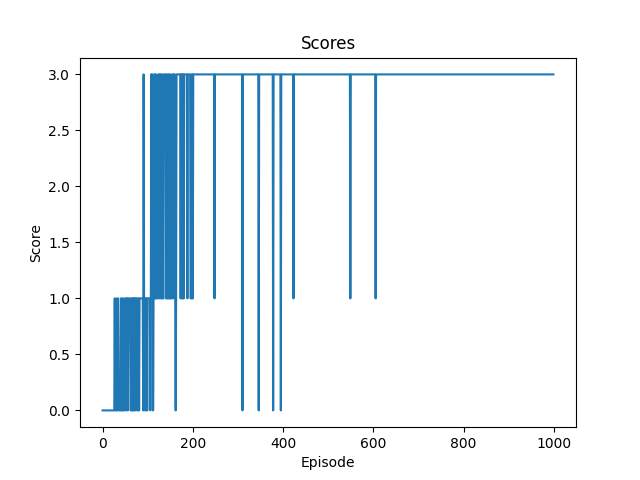
\includegraphics[width=0.8\textwidth]{level1.png}
\caption{Q-Learning on Level 1}
\end{figure}

\subsubsection{Level 3}
Similarly, the algorithm's performance on Level 3 was evaluated. 
The graph below illustrates the algorithm's adaptability and learning progression at this more complex level.

\begin{figure}[h]
\centering
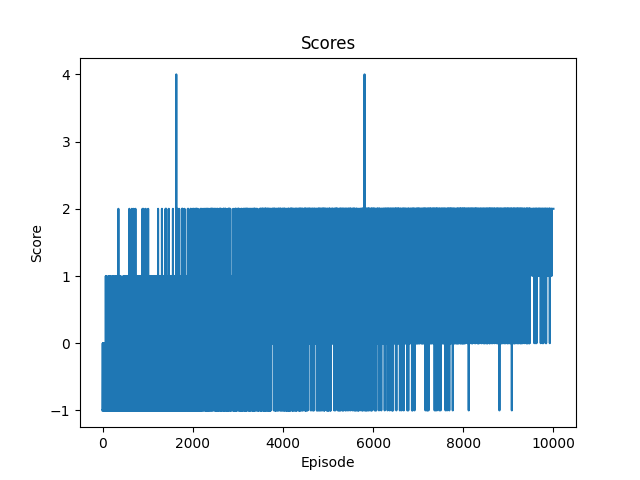
\includegraphics[width=0.8\textwidth]{level3.png}
\caption{Q-Learning on Level 3}
\end{figure}

\subsubsection{Level 6}
For this level, we get a memory error at qtable creation.

\section{Analysis}
\subsection{Level 1 Convergence}
In the case of Level 1, the Q-Learning algorithm successfully converged to an optimal policy after approximately 200 episodes. This level, with its relatively simple layout and fewer challenges, allowed the algorithm to efficiently explore and exploit the environment, learning the optimal actions within a reasonable number of episodes.

\subsection{Level 3 Challenges}
Contrastingly, Level 3 presented a more complex scenario with 
increased challenges, including the presence of multiple agents and potentially
 more dynamic elements like lasers. 
 Despite running for over 10,000 episodes, 
 the algorithm showed progress but did not converge to a stable policy.
  This lack of convergence could be attributed to several factors:

\begin{itemize}
    \item \textbf{Multiple Agents:} The introduction of an additional agent increases the complexity of the state space exponentially. This complexity might have made it difficult for the algorithm to consistently predict the outcomes of actions, leading to less effective learning.
    \item \textbf{Dynamic Elements:} Elements like lasers introduce additional uncertainty and complexity to the environment, which can significantly impact the learning process and make convergence more challenging.
    \item \textbf{Parameterization:} The automatic parameterization
     of the Q-agents, while designed to be adaptive, may not have been optimal
      for the complexities introduced in Level 3. 
      Inadequate tuning of parameters could be hindering the learning process.
    \item \textbf{Features:} The features used to adapt the Q-agents may not be 
    sufficient to capture the complexity of the environment.
    \end{itemize}

These observations suggest that while Q-Learning is effective in simpler 
scenarios, its application in more complex environments requires careful consideration
 of the factors mentioned above. Future work could involve experimenting with supplementary features like the balanced greedy traveling salesmen problem algorithm used in the projects 1 and 2.

\section{Conclusion}
This project offered deep insights into the dynamics of reinforcement learning algorithms in MDPs. 
It highlighted the strengths and weaknesses of Value Iteration and Q-Learning, 
providing a clear understanding of their applicability in different scenarios.

\section{Tools}
\begin{itemize}
    \item Python
    \item Numpy
    \item Matplotlib
    \item ChatGPT
    \item Github Copilot
\end{itemize}
\section{References}
\bibliographystyle{plain}
\bibliography{references}

\end{document}
